\chapter{जनन का हॉर्मोनी नियंत्रण}\label{ch:b2:reproductive-hormones}

हर महीने, तीस वर्ष तक एक-दो दिन की परिशुद्धता से बँधी समय-सारणी पर,
एक \omterm{def:b2:mammal-reproduction:ovary}{पुटक} पकता है, एक अंडाणु छोड़ा जाता है, गर्भाशय का अस्तर
बनाया जाता है और फिर, जब तक कोई भ्रूण न आ पहुँचे, ढहा दिया जाता है।
शरीर की कोई घड़ी इस दर से नहीं टिकती; वह लय तीन अंगों --- अधश्चेतक,
पीयूष और अंडाशय --- के बीच की बातचीत से उभरती है, जिसमें हर हॉर्मोन
अगले का मोचन नियंत्रित करता है और अंतिम पहले को। यह अध्याय
उस बातचीत को खोलकर रखता है: वह अक्ष जो दोनों लिंग चलाती है,
\omterm{def:b2:mammal-reproduction:testis}{वृषण} का अविराम नियंत्रण, अंडाशय का चक्रीय नियंत्रण अपने उस
उल्लेखनीय ऋण-से-धन प्रतिपुष्टि स्विच सहित, और वे रास्ते जिनसे उस अक्ष
पर गर्भावस्था, औषधियाँ और चिकित्सालय हावी हो जाते हैं।

\section{अक्ष}

\begin{definition}[अधश्चेतक-पीयूष-जनद अक्ष]\label{def:b2:reproductive-hormones:axis}
\index{गोनैडोट्रोपिन-मोचक हॉर्मोन}\index{ल्यूटीनकारी हॉर्मोन}\index{पुटक-उद्दीपक हॉर्मोन}\index{ऋण प्रतिपुष्टि!हॉर्मोनी}
\emph{अधश्चेतक} के न्यूरॉन \emph{GnRH}
(गोनैडोट्रोपिन-मोचक हॉर्मोन, दस ऐमीनो अम्लों का एक पेप्टाइड) को उन छोटी
प्रवेशिका वाहिकाओं में स्रावित करते हैं जो \emph{अग्र पीयूष} तक जाती
हैं, और वह भी हर एक-दो घंटे पर छोटी-छोटी \emph{स्पंदों} में। GnRH
पीयूष से दो ग्लाइकोप्रोटीन हॉर्मोन सामान्य परिसंचरण में स्रावित कराती
है, यानी \emph{गोनैडोट्रोपिन} \emph{LH} (ल्यूटीनकारी
हॉर्मोन) और \emph{FSH} (पुटक-उद्दीपक हॉर्मोन)। ये \emph{जनदों} पर काम
करते हैं: LH स्टेरॉइड बनाने वाली कोशिकाओं पर (\omterm{def:b2:mammal-reproduction:testis}{लाइडिग कोशिकाएँ},
थीका और पीत कोशिकाएँ), और FSH उन कोशिकाओं पर जो युग्मकों की परिचर्या
करती हैं (सर्टोली और कणिकामय कोशिकाएँ)। जनद स्टेरॉइडों से उत्तर देते
हैं --- \emph{टेस्टोस्टेरोन}, \emph{एस्ट्राडायोल},
\emph{प्रोजेस्टेरोन} --- और पेप्टाइड \emph{इनहिबिन} से, और ये
अधश्चेतक तथा पीयूष पर प्रतिपुष्टि करते हैं: स्टेरॉइड दोनों पर, अधिकतर
\emph{ऋणात्मक} रूप से; और इनहिबिन केवल FSH पर। परिणाम एक नियमित
चक्र है जिसमें जनद का निर्गत किसी नियत बिंदु पर रखा जाता है, और यही
तीन-तल्ला अभिकल्प अवटु ग्रंथि तथा अधिवृक्क वल्कुट भी चलाता है। ये
हॉर्मोन अपनी कोशिकाओं पर जिन क्रियाविधियों से काम करते हैं वे
\cref{ch:b2:cell-signalling} का विषय हैं।
\end{definition}

\begin{omfigure}
\begin{tikzpicture}[every node/.style={font=\scriptsize}, >=stealth]
  \node[draw, rounded corners, fill=omDef!15, align=center, minimum width=3cm] (hyp) at (0,4.2) {अधश्चेतक\\GnRH, स्पंदों में};
  \node[draw, rounded corners, fill=omDef!15, align=center, minimum width=3cm] (pit) at (0,2.2) {अग्र पीयूष\\LH और FSH};
  \node[draw, rounded corners, fill=omProp!20, align=center, minimum width=3cm] (gon) at (0,0) {जनद\\स्टेरॉइड, इनहिबिन};
  \node[draw, rounded corners, fill=omExo!25, align=center, minimum width=3cm] (tar) at (5.2,0) {लक्ष्य ऊतक\\युग्मकजनन, नलिकाएँ,\\गौण लक्षण};
  \draw[->, thick] (hyp) -- (pit) node[midway, right] {प्रवेशिका वाहिकाएँ};
  \draw[->, thick] (pit) -- (gon) node[midway, right] {रक्त};
  \draw[->, thick] (gon) -- (tar);
  \draw[->, thick, omThm] (gon.west) .. controls (-3.0,0) and (-3.0,2.2) .. (pit.west);
  \draw[->, thick, omThm] (gon.west) .. controls (-4.6,0) and (-4.6,4.2) .. (hyp.west);
  \node[omThm, anchor=east, align=right] at (-3.9,1.2) {पीयूष तक:\\स्टेरॉइड $(-)$,\\FSH पर इनहिबिन $(-)$};
  \node[omThm, anchor=east, align=right] at (-3.9,3.6) {अधश्चेतक तक:\\स्टेरॉइड $(-)$\\(चक्र के मध्य में\\एस्ट्राडायोल $(+)$)};
\end{tikzpicture}

{\small वह अक्ष: अधश्चेतकी GnRH पीयूष की LH और FSH चलाती है,
जो जनद को चलाती हैं; और जनद के स्टेरॉइड तथा इनहिबिन दोनों ऊपरी तल्लों पर
ऋणात्मक प्रतिपुष्टि करते हैं --- सिवाय एस्ट्राडायोल की उस छोटी धन
प्रतिपुष्टि के जो \omterm{def:b2:mammal-reproduction:ovary}{अंडोत्सर्ग} का चालक है।}
\end{omfigure}

\begin{proposition}[स्पंद क्यों मायने रखते हैं]\label{prop:b2:reproductive-hormones:pulses}
\index{स्पंदी स्राव}\index{ग्राही असंवेदन}
पीयूष GnRH को तभी उत्तर देता है जब वह स्पंदों में आए। जो कोशिका
किसी हॉर्मोन के सामने लगातार रहे वह उस हॉर्मोन के ग्राही अपनी सतह से
हटा देती है (\emph{असंवेदन}); और यदि ग्राही-कोष $s$ दर से भरता हो,
$d$ आधारी दर से हटता हो और, हॉर्मोन $H$ की उपस्थिति में, $iH$ अतिरिक्त
दर से, तो
\[
\frac{\mathrm{d}R}{\mathrm{d}t} = s - (d + iH)\,R, \qquad R^* = \frac{s}{d + iH},
\]
यानी लगातार ऊँची $H$ ग्राही-संख्या को किसी नीची स्थायी अवस्था तक ले
जाती है और कोशिका चुप हो जाती है, जबकि हॉर्मोन-रहित अंतरालों से अलग
की गई छोटी स्पंदें उस कोष को उनके बीच उबरने देती हैं
(काल-नियतांक $1/d$)। हर नब्बे मिनट पर एक GnRH स्पंद
पीयूष को उत्तरदायी रखती है; जबकि कोई अचर निवेश, या कोई
दीर्घक्रिय GnRH प्रचालक, उसे दिनों में बंद कर देता है --- और यही उन
औषधियों का आधार है जो प्रोस्टेट कैंसर, अंतर्गर्भाशयकलाभ्रंश और
असामयिक यौवनारंभ में उस अक्ष को दबाती हैं। स्पंद-बारंबारता सूचना भी
कूटबद्ध करती है: तेज़ स्पंदें LH के पक्ष में हैं, धीमी स्पंदें FSH के।
\end{proposition}
\begin{proof}[प्रमाण-सामग्री]
नोबिल (1978--1980) ने रीसस बंदरों के GnRH न्यूरॉन नष्ट कर दिए,
जिससे LH, FSH और वह चक्र मिट गए, और फिर GnRH को पंप से
लौटाया: घंटे में एक स्पंद ने गोनैडोट्रोपिन तथा सामान्य
अंडोत्सर्गी चक्र बहाल कर दिए; वही दैनिक मात्रा लगातार देने पर वे कुछ
दिन बहाल रहे और फिर LH तथा FSH गिरकर शून्य हो गए; और स्पंदों पर
लौटने से वे फिर बहाल हो गए। संकेत वह मात्रा नहीं, पहुँचाने का ढंग है।
\end{proof}

\begin{omfigure}
\begin{tikzpicture}
\begin{axis}[
  width=0.8\linewidth, height=5.4cm,
  axis x line=bottom, axis y line=left,
  xmin=0, xmax=40, ymin=0, ymax=1.2,
  xlabel={दिन}, ylabel={प्लाज़्मा LH (सापेक्ष)},
  xlabel style={font=\small, at={(axis description cs:0.5,-0.13)}, anchor=north},
  ylabel style={font=\small},
  tick label style={font=\small}, xtick={0,10,20,30,40}, ytick={0,0.5,1},
  clip=false,
]
\addplot[very thick, omDef, domain=0:10, samples=2] {1};
\addplot[very thick, omThm, domain=10:25, samples=60] {exp(-(x-10)/3)};
\addplot[very thick, omDef, domain=25:40, samples=60] {1-exp(-(x-25)/2)};
\fill[omDef!15] (axis cs:0,1.05) rectangle (axis cs:10,1.15); \node[font=\scriptsize] at (axis cs:5,1.1) {प्रति घंटा स्पंदें};
\fill[omThm!15] (axis cs:10,1.05) rectangle (axis cs:25,1.15); \node[font=\scriptsize] at (axis cs:17.5,1.1) {सतत निवेश};
\fill[omDef!15] (axis cs:25,1.05) rectangle (axis cs:40,1.15); \node[font=\scriptsize] at (axis cs:32.5,1.1) {फिर स्पंदें};
\end{axis}
\end{tikzpicture}

{\small नोबिल का प्रयोग, आरेखी रूप में। जिस बंदर के अपने
GnRH न्यूरॉन नष्ट कर दिए गए हों उसमें GnRH की प्रति घंटा स्पंदें LH
बनाए रखती हैं; उतनी ही दैनिक मात्रा के सतत निवेश पर आने से
वह दिनों में बुझ जाती है, और स्पंदें उसे फिर बहाल कर देती हैं।}
\end{omfigure}

\begin{omfigure}
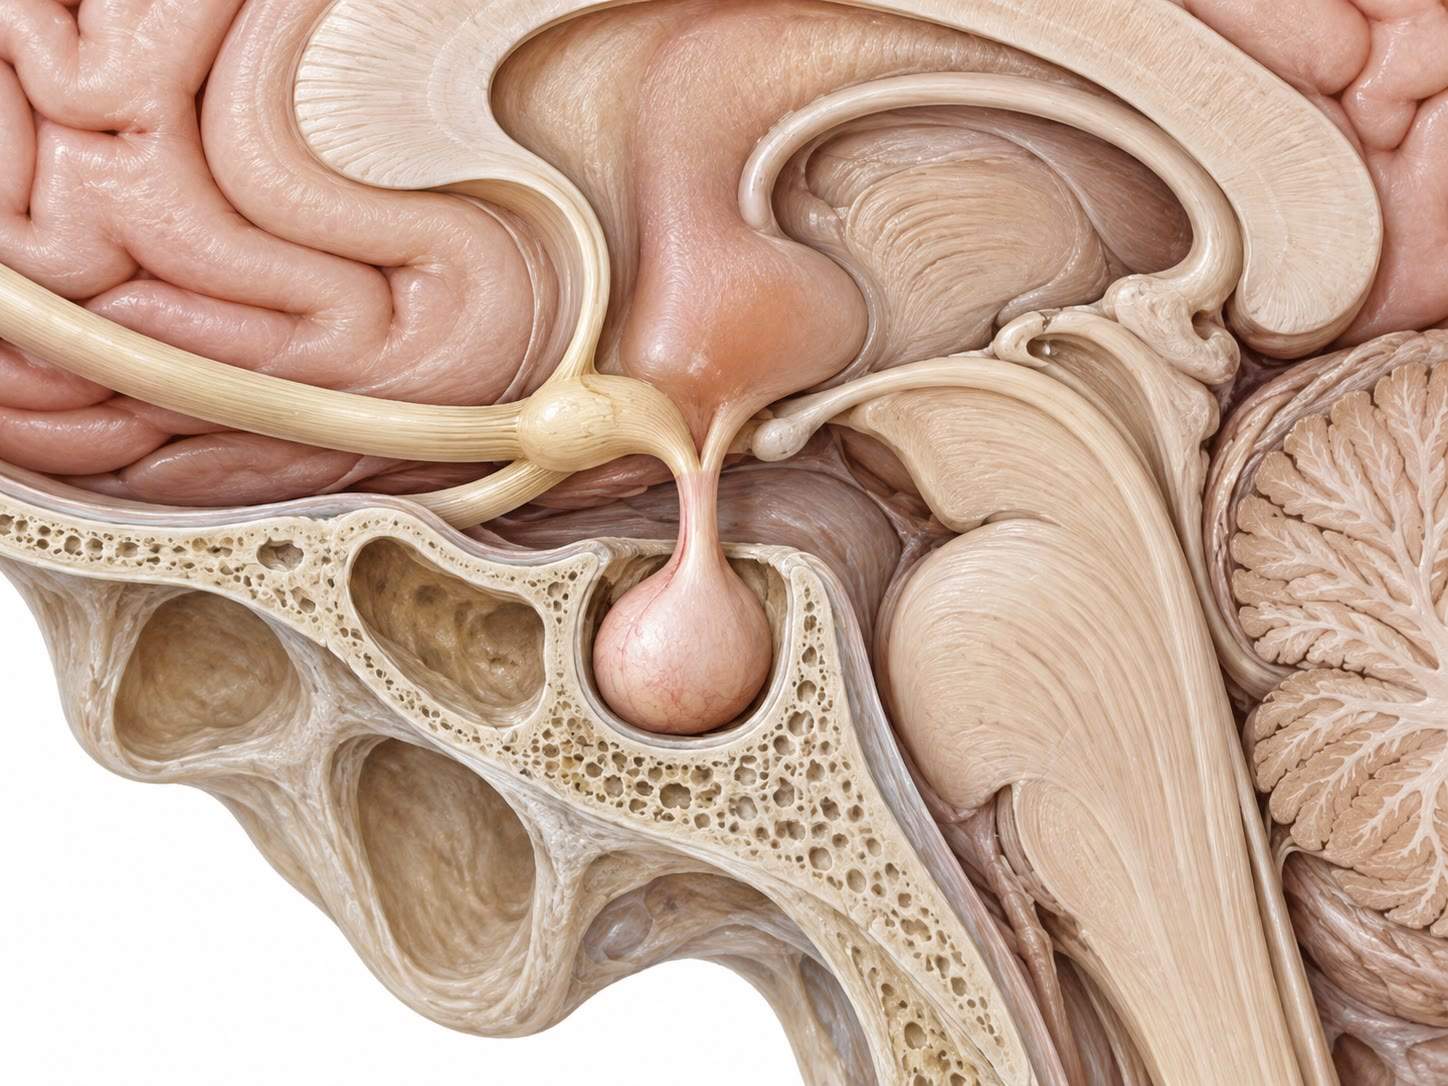
\includegraphics[width=0.55\linewidth]{images/book4/ai/b4-09-hypothalamus-pituitary.jpg}

{\small मस्तिष्क का आधार, धनु काट में: ऊपर अधश्चेतक,
वृंत, और अपनी अस्थि-कोटर में पीयूष --- यानी उस अक्ष का साज-सामान।}
\end{omfigure}

\section{नर: अविराम नियंत्रण}

\begin{proposition}[वृषण का नियंत्रण]\label{prop:b2:reproductive-hormones:testis}
\index{टेस्टोस्टेरोन}\index{इनहिबिन}
LH \omterm{def:b2:mammal-reproduction:testis}{लाइडिग कोशिकाओं} पर काम करती है, जो \emph{टेस्टोस्टेरोन} बनाती हैं
(किसी वयस्क पुरुष के रक्त में \qtyrange{3}{10}{ng/mL}, और \omterm{def:b2:mammal-reproduction:testis}{वृषण}
के भीतर सौ गुना अधिक)। FSH \omterm{def:b2:mammal-reproduction:testis}{सर्टोली कोशिकाओं} पर काम करती है, जो
--- वहीं के टेस्टोस्टेरोन के साथ --- \omterm{def:b2:mammal-reproduction:testis}{शुक्राणुजनन} सँभालती हैं और
\emph{इनहिबिन} स्रावित करती हैं। टेस्टोस्टेरोन अधश्चेतक
और पीयूष पर प्रतिपुष्टि करके LH नीची रखता है; और इनहिबिन पीयूष पर
प्रतिपुष्टि करके FSH नीची रखती है। दोनों चक्र \emph{ऋणात्मक} हैं और वह
तंत्र \emph{अविराम} है: हॉर्मोन-स्तर स्पंदों के साथ और दिन के साथ
उतार-चढ़ाव करते हैं (सुबह सबसे ऊँचे) पर चक्र नहीं चलाते, और शुक्राणु
लगातार बनते रहते हैं। टेस्टोस्टेरोन सहायक ग्रंथियाँ और नलिकाएँ, दाढ़ी,
आवाज़, पेशी तथा अस्थि, लाल-कोशिका उत्पादन और कामेच्छा भी गढ़ता और बनाए
रखता है, और भ्रूण में उसी ने नर काया बनाई थी
(\cref{ch:b2:mammal-reproduction})। बधियाकरण उसे हटा देता है: प्रतिपुष्टि
न रहने से LH और FSH कई गुना चढ़ जाती हैं, और गौण लक्षण क्षीण हो जाते
हैं; और इंजेक्ट किया गया टेस्टोस्टेरोन उन लक्षणों को लौटा देता है
--- पर उर्वरता नहीं, क्योंकि वह LH को भी दबा देता है और इसलिए उस
वृषण-भीतरी टेस्टोस्टेरोन को भी जो \omterm{def:b2:mammal-reproduction:testis}{शुक्राणुजनन} को चाहिए। इसीलिए
उपचयी स्टेरॉइड पुरुषों को बंध्य बना देते हैं।
\end{proposition}
\begin{proof}[प्रमाण-सामग्री]
बर्थोल्ड (1849) ने मुर्ग़ों का बधियाकरण किया: उनकी कलगियाँ सिकुड़ गईं और
वे न बाँग देते थे न लड़ते थे। किसी बधिया मुर्ग़े के उदर में ग्राफ़्ट
किया गया कोई \omterm{def:b2:mammal-reproduction:testis}{वृषण}, जिसे नई रक्त-आपूर्ति तो मिली पर तंत्रिकाएँ नहीं,
कलगी, बाँग और लड़ाई लौटा लाया: यानी \omterm{def:b2:mammal-reproduction:testis}{वृषण} ने रक्त के रास्ते काम किया ---
और यह किसी आंतरिक स्राव का पहला प्रदर्शन था, हॉर्मोन शब्द से पचास वर्ष
पहले। टेस्टोस्टेरोन 1935 में अलग किया और संश्लेषित किया गया।
\end{proof}

\section{मादा: एक स्विच वाला चक्र}

\begin{definition}[अंडाशयी और गर्भाशयी चक्र]\label{def:b2:reproductive-hormones:cycle}
\index{रजोचक्र}\index{पुटकीय प्रावस्था}\index{पीत प्रावस्था}\index{LH उछाल}\index{गर्भाशय अंतःस्तर}
वह चक्र रजःस्राव के पहले दिन से गिना जाता है और लगभग 28 दिन चलता है।
\emph{पुटकीय प्रावस्था} (दिन 1--14): FSH, जो पिछले \omterm{def:b2:mammal-reproduction:ovary}{पीत पिंड} की
मृत्यु से प्रतिपुष्टि-मुक्त हो चुकी है, \omterm{def:b2:mammal-reproduction:ovary}{पुटकों} का एक दल भर्ती
करती है; वे \emph{एस्ट्राडायोल} स्रावित करते हैं, जो लगातार चढ़ता है;
एस्ट्राडायोल और इनहिबिन FSH नीची करते हैं, और उस गिरावट को केवल वही
\omterm{def:b2:mammal-reproduction:ovary}{पुटक} झेल पाता है जिसके FSH ग्राही सबसे अधिक हैं --- यानी प्रबल \omterm{def:b2:mammal-reproduction:ovary}{पुटक}।
गर्भाशय में एस्ट्राडायोल \emph{गर्भाशय अंतःस्तर} फिर गढ़ता है (यानी
प्रसारी प्रावस्था) और ग्रीवा का श्लेष्म पतला करता है। \emph{\omterm{def:b2:mammal-reproduction:ovary}{अंडोत्सर्ग}}
(दिन 14): जब एस्ट्राडायोल डेढ़ दिन तक लगभग \qty{200}{pg/mL} से ऊपर बना
रहे, तब अधश्चेतक तथा पीयूष पर उसकी प्रतिपुष्टि
ऋणात्मक से \emph{धनात्मक} हो जाती है; LH एक दिन में दस गुना चढ़ती है
--- यानी \emph{LH उछाल} --- और उसके आरंभ के लगभग 36 घंटे बाद
\omterm{def:b2:mammal-reproduction:ovary}{पुटक} फटता है और अंडाणुक छोड़ देता है। \emph{पीत प्रावस्था} (दिन
15--28): ख़ाली हुआ \omterm{def:b2:mammal-reproduction:ovary}{पुटक} \omterm{def:b2:mammal-reproduction:ovary}{पीत पिंड} बन जाता है, जो
LH के नीचे \emph{प्रोजेस्टेरोन} (\qtyrange{10}{20}{ng/mL}) और
एस्ट्राडायोल स्रावित करता है; प्रोजेस्टेरोन गर्भाशय अंतःस्तर को स्रावी
बना देता है, श्लेष्म गाढ़ा करता है, आधारी देह-ताप \qty{0.3}{\celsius}
चढ़ा देता है, और एस्ट्राडायोल के साथ मिलकर LH तथा FSH दबा देता है।
\omterm{def:b2:mammal-reproduction:ovary}{पीत पिंड} की आयु लगभग 14 दिन है; और जब तक किसी भ्रूण की hCG उसे न बचा
ले, वह क्षीण हो जाता है, प्रोजेस्टेरोन तथा एस्ट्राडायोल गिरते हैं,
गर्भाशय अंतःस्तर झड़ जाता है (\emph{रजःस्राव}), FSH चढ़ती है, और अगला
चक्र आरंभ हो जाता है। पीत प्रावस्था 14 दिन पर नियत है; चक्र की लंबाई
में जो भी भिन्नता है वह पुटकीय प्रावस्था की भिन्नता है।
\end{definition}

\begin{omfigure}
\begin{tikzpicture}
\begin{axis}[
  width=0.94\linewidth, height=6.4cm,
  axis x line=bottom, axis y line=left,
  xmin=0, xmax=28, ymin=0, ymax=1.15,
  xlabel={चक्र का दिन}, ylabel={हॉर्मोन (शिखर के सापेक्ष)},
  xlabel style={font=\small, at={(axis description cs:0.5,-0.11)}, anchor=north},
  ylabel style={font=\small},
  tick label style={font=\small}, xtick={0,7,14,21,28}, ytick={0,0.5,1},
  legend style={font=\scriptsize, at={(0.5,-0.25)}, anchor=north, draw=none, legend columns=4},
  clip=false,
]
\addplot[very thick, omThm, domain=0:28, samples=120] {0.1 + 0.9*exp(-((x-14)^2)/0.9)};
\addlegendentry{LH}
\addplot[very thick, omProp, domain=0:28, samples=120] {0.35*exp(-x/6) + 0.15 + 0.35*exp(-((x-14)^2)/1.2)};
\addlegendentry{FSH}
\addplot[very thick, omDef, domain=0:28, samples=160] {0.1 + 0.9*exp(-((x-12.5)^2)/6) + 0.4*exp(-((x-21)^2)/12)};
\addlegendentry{एस्ट्राडायोल}
\addplot[very thick, omExo!70!black, domain=0:28, samples=160] {0.03 + 0.97*exp(-((x-21)^2)/12)*(x>14)};
\addlegendentry{प्रोजेस्टेरोन}
\draw[dashed, gray] (axis cs:14.5,0) -- (axis cs:14.5,1.1); \node[font=\scriptsize, anchor=south] at (axis cs:14.5,1.1) {अंडोत्सर्ग};
\node[font=\scriptsize, anchor=north] at (axis cs:7,1.1) {पुटकीय प्रावस्था};
\node[font=\scriptsize, anchor=north] at (axis cs:21.5,1.1) {पीत प्रावस्था};
\end{axis}
\end{tikzpicture}

{\small चक्र के हॉर्मोन। बढ़ते \omterm{def:b2:mammal-reproduction:ovary}{पुटक} का एस्ट्राडायोल
\omterm{def:b2:reproductive-hormones:cycle}{पुटकीय प्रावस्था} भर चढ़ता है और, किसी देहली के पार जाकर,
\omterm{def:b2:reproductive-hormones:cycle}{LH उछाल} का चालक बनता है; \omterm{def:b2:mammal-reproduction:ovary}{अंडोत्सर्ग} लगभग 36 घंटे बाद होता है; और फिर
\omterm{def:b2:mammal-reproduction:ovary}{पीत पिंड} पखवाड़े भर प्रोजेस्टेरोन स्रावित करके मर जाता है।}
\end{omfigure}

\begin{omfigure}
\begin{tikzpicture}[every node/.style={font=\scriptsize}]
  % endometrium thickness over the cycle
  \draw[thick, ->] (0,0) -- (12.4,0) node[right] {दिन};
  \foreach \x/\l in {0/1, 2.1/5, 6.0/14, 12/28} \draw (\x,0.08) -- (\x,-0.08) node[below] {\l};
  \fill[omThm!25] (0,0) -- (0,1.4) .. controls (0.8,1.2) and (1.6,0.5) .. (2.1,0.35) -- (2.1,0) -- cycle;
  \fill[omDef!20] (2.1,0) -- (2.1,0.35) .. controls (3.5,0.6) and (5.2,1.3) .. (6.0,1.5) -- (6.0,0) -- cycle;
  \fill[omExo!35] (6.0,0) -- (6.0,1.5) .. controls (8,1.8) and (11,1.9) .. (12,1.6) -- (12,0) -- cycle;
  \node at (1.0,1.8) {रजःस्राव};
  \node at (4.0,1.8) {प्रसारी (एस्ट्राडायोल)};
  \node at (9,2.2) {स्रावी (प्रोजेस्टेरोन): ग्रंथियाँ, ग्लाइकोजन, कुंडलित धमनियाँ};
  \node[anchor=east] at (-0.1,0.8) {गर्भाशय अंतःस्तर};
\end{tikzpicture}

{\small गर्भाशयी चक्र। \omterm{def:b2:reproductive-hormones:cycle}{गर्भाशय अंतःस्तर} रजःस्राव पर झाड़ दिया जाता है,
एस्ट्राडायोल के नीचे फिर गढ़ा जाता है, और प्रोजेस्टेरोन के नीचे स्रावी
बनाया जाता है, ताकि दिन 21 के आसपास कोई कोरकपुटी ग्रहण कर सके; और
प्रोजेस्टेरोन गिरते ही वह फिर झाड़ दिया जाता है।}
\end{omfigure}

\begin{omfigure}
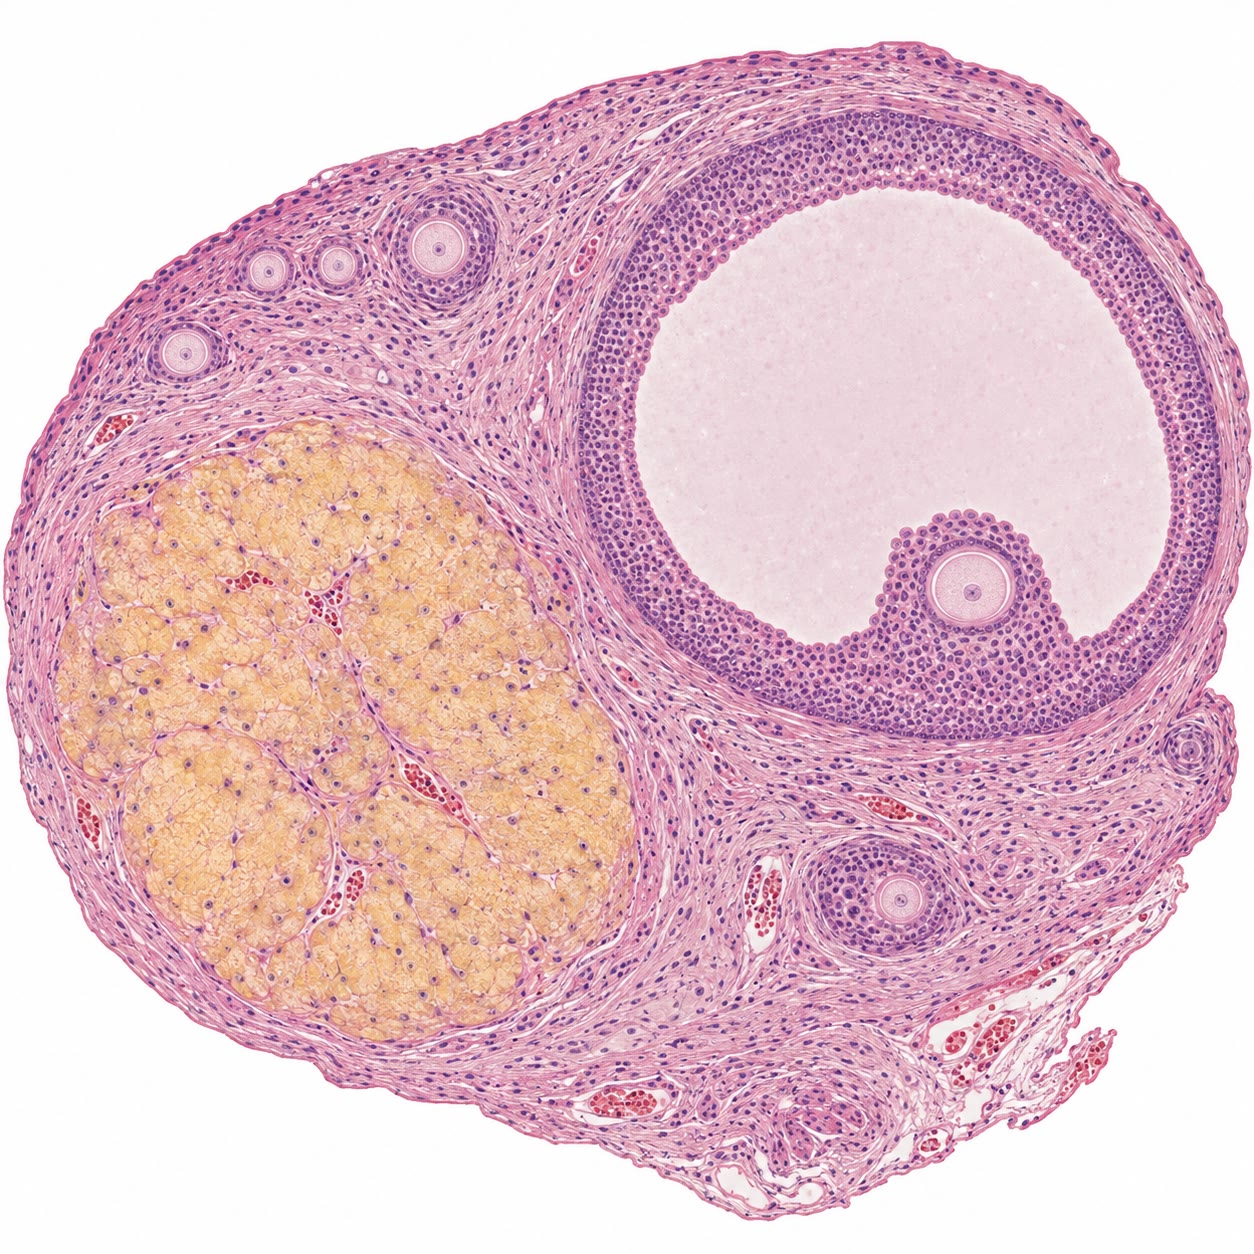
\includegraphics[width=0.46\linewidth]{images/book4/ai/b4-09-ovary-histology.jpg}

{\small काट में एक अंडाशय: गुहा और अंडाणुक सहित एक परिपक्व \omterm{def:b2:mammal-reproduction:ovary}{पुटक},
सतह के नीचे छोटे आद्य \omterm{def:b2:mammal-reproduction:ovary}{पुटक}, और किसी पिछले चक्र का एक \omterm{def:b2:mammal-reproduction:ovary}{पीत
पिंड}।}
\end{omfigure}

\begin{theorem}[ऋण से धन प्रतिपुष्टि तक का स्विच]\label{thm:b2:reproductive-hormones:switch}
\index{धन प्रतिपुष्टि!LH उछाल}
आरंभिक \omterm{def:b2:reproductive-hormones:cycle}{पुटकीय प्रावस्था} के नीचे स्तरों पर एस्ट्राडायोल
LH और FSH को संदमित करता है; और लगभग \qty{200}{pg/mL} से ऊपर का
एस्ट्राडायोल, यदि लगभग \qty{36}{h} से अधिक बना रहे, तो उलटा करता है:
वह अधश्चेतक से GnRH का एक उछाल छुड़वाता है और पीयूष से उसका उत्तर
LH की दस गुनी चढ़ाई के रूप में दिलवाता है। क्रियाविधि चिह्न का परिवर्तन
है, परिमाण का नहीं: कोई ऊँची, टिकाऊ मात्रा पीयूष में LH का एक
बड़ा भंडार और GnRH के प्रति बढ़ी हुई संवेदिता उत्पन्न करती है, और
अधश्चेतक में (किसपेप्टिन न्यूरॉनों के रास्ते) GnRH स्पंद-जनित्र को
उछाल-विधा पर डाल देती है। वह स्विच किसी क्रमिक संकेत को --- कि
\omterm{def:b2:mammal-reproduction:ovary}{पुटक} कितना एस्ट्राडायोल बनाता है --- दिन भर की परिशुद्धता से
सधी सर्वथा-अथवा-कुछ नहीं घटना में बदल देता है, और \omterm{def:b2:mammal-reproduction:ovary}{अंडोत्सर्ग}
को यही चाहिए; और चूँकि केवल कोई बड़ा, परिपक्व \omterm{def:b2:mammal-reproduction:ovary}{पुटक} ही
\qty{200}{pg/mL} बनाए रख सकता है, वह उछाल तभी छूटती है जब छोड़ने को कोई
अंडाणु तैयार हो। एक बार \omterm{def:b2:mammal-reproduction:ovary}{अंडोत्सर्ग} हो जाने पर \omterm{def:b2:mammal-reproduction:ovary}{पीत पिंड} का
प्रोजेस्टेरोन ऋण प्रतिपुष्टि लौटा देता है और कोई दूसरी उछाल नहीं
आती।
\end{theorem}
\begin{proof}[प्रमाण-सामग्री]
जिन स्त्रियों और बंदरों की अक्ष दबा दी गई हो, उनमें
एस्ट्राडायोल का ऐसा निवेश जो प्लाज़्मा-स्तर को दो दिन \qty{200}{pg/mL}
से ऊपर चढ़ा दे, उसके बाद एक \omterm{def:b2:reproductive-hormones:cycle}{LH उछाल} आती है; पर उतनी ही मात्रा एक
दिन दी जाए, या तीन दिन नीचा स्तर रखा जाए, तो नहीं। उस निवेश से पहले
दिया गया प्रोजेस्टेरोन उस उछाल को रोक देता है; और साथ दिया जाए तो उसे
पहले ले आता और बढ़ा देता है। मात्रा और अवधि की वह देहली प्राकृतिक
एस्ट्राडायोल-चढ़ाई से प्राकृतिक उछाल के समय को फिर से बना देती है।
\end{proof}

\section{चक्र पर हावी होना}

\begin{proposition}[गर्भावस्था, स्तनपायन, रजोनिवृत्ति]\label{prop:b2:reproductive-hormones:overrides}
\index{मानव जरायु गोनैडोट्रोपिन}\index{रजोनिवृत्ति}
कोई रोपित होता भ्रूण \emph{hCG} स्रावित करता है, यानी LH जैसा कोई
हॉर्मोन जो LH ग्राही से बँधता है और \omterm{def:b2:mammal-reproduction:ovary}{पीत पिंड} को उसके चौदह दिनों
से आगे भी जीवित तथा स्रावी रखता है; और सप्ताह दस तक \omterm{def:b2:mammal-reproduction:placenta}{अपरा} स्वयं
गर्भावस्था बनाए रखने लायक़ प्रोजेस्टेरोन तथा एस्ट्रोजन बना लेती है
और \omterm{def:b2:mammal-reproduction:ovary}{पीत पिंड} की ज़रूरत नहीं रहती। पूरी गर्भावस्था में ऊँचे
स्टेरॉइड LH और FSH को शून्य पर रखते हैं: कोई \omterm{def:b2:mammal-reproduction:ovary}{पुटक} नहीं बढ़ता, कोई
\omterm{def:b2:mammal-reproduction:ovary}{अंडोत्सर्ग} नहीं होता। जन्म के बाद चूसना प्रोलैक्टिन चढ़ाता है और GnRH
स्पंदें धीमी कर देता है, इसलिए \omterm{def:b2:mammal-reproduction:ovary}{अंडोत्सर्ग} महीनों दबा रहता है।
\emph{रजोनिवृत्ति} पर \omterm{def:b2:mammal-reproduction:ovary}{पुटकों} का भंडार चुक जाता है: एस्ट्राडायोल और
इनहिबिन गिरते हैं, और प्रतिपुष्टि करने को कुछ न रहने से LH तथा FSH
अपने पहले स्तर के दस गुने तक चढ़ जाती हैं और वहीं बनी रहती हैं --- यानी
उस ग्रंथि का चिह्न जिसने उत्तर देना छोड़ दिया है।
\end{proposition}

\begin{proposition}[गर्भनिरोध और सहायित जनन]\label{prop:b2:reproductive-hormones:clinic}
\index{गर्भनिरोध!हॉर्मोनी}\index{पात्रे निषेचन}
संयुक्त गोली रोज़ एक संश्लिष्ट एस्ट्रोजन और एक प्रोजेस्टिन पहुँचाती है:
अचर स्टेरॉइड-स्तर FSH तथा LH नीची रखता है, कोई
\omterm{def:b2:mammal-reproduction:ovary}{पुटक} भर्ती नहीं होता, कोई एस्ट्राडायोल-चढ़ाई नहीं होती, और वह उछाल
कभी नहीं छूटती; और वह प्रोजेस्टिन ग्रीवा का श्लेष्म भी गाढ़ा कर देता है।
सात दिन का विराम \omterm{def:b2:reproductive-hormones:cycle}{गर्भाशय अंतःस्तर} को रक्तस्राव करने देता है; और
लगातार दो से अधिक दिन गोलियाँ छूट जाएँ तो FSH बच निकलती है और कोई
\omterm{def:b2:mammal-reproduction:ovary}{पुटक} बढ़ सकता है। आपात गर्भनिरोध किसी बड़ी प्रोजेस्टिन मात्रा से उस
उछाल को कुछ दिन टाल देता है। \emph{\omterm{prop:b2:reproductive-hormones:clinic}{पात्रे निषेचन}} में उस अक्ष को
उलटी दिशा में चलाया जाता है: दस दिन रोज़ दी गई FSH किसी एक प्रबल
\omterm{def:b2:mammal-reproduction:ovary}{पुटक} के चुनाव पर हावी हो जाती है और दस या अधिक पका देती है; कोई
GnRH प्रतिरोधी किसी असमय स्वतःस्फूर्त उछाल को रोकता है; hCG का एक
इंजेक्शन उस उछाल की जगह ले लेता है, और अंडाणुक 34 से 36 घंटे बाद, ठीक
उनके छोड़े जाने से पहले, एकत्र कर लिए जाते हैं; वे तश्तरी में निषेचित
किए जाते हैं और एक या दो भ्रूण स्थानांतरित कर दिए जाते हैं तथा
बाक़ी जमा दिए जाते हैं। पुरुषों में बाहर से दिया गया टेस्टोस्टेरोन या
कोई GnRH अनुरूपी LH दबाकर \omterm{def:b2:mammal-reproduction:testis}{शुक्राणुजनन} दबा देता है --- और यही किसी
नर हॉर्मोनी गर्भनिरोधक का सिद्धांत है, जो अब तक बाज़ार में नहीं आया।
यह सब पहले खंड की वही अक्ष है, उलटी पढ़ी हुई।
\end{proposition}

\section{अभ्यास}

\begin{exercise}[$\star$]\label{exo:b2:reproductive-hormones:1}
नर के लिए वह अक्ष खींचिए: तीनों तल्ले, चारों हॉर्मोन, दोनों
प्रतिपुष्टि चक्र, और वे कोशिकाएँ जिन पर हर हॉर्मोन काम करता है।
\end{exercise}

\begin{exercise}[$\star$]\label{exo:b2:reproductive-hormones:2}
अंडाशयी और गर्भाशयी चक्रों की प्रावस्थाएँ उनके दिनों सहित दीजिए, और
वह हॉर्मोन भी जो हर एक पर छाया रहता है।
\end{exercise}

\begin{exercise}[$\star$]\label{exo:b2:reproductive-hormones:3}
समझाइए कि संयुक्त गोली \omterm{def:b2:mammal-reproduction:ovary}{अंडोत्सर्ग} कैसे रोकती है, और गोली-रहित सप्ताह
में रक्तस्राव क्यों होता है।
\end{exercise}

\begin{exercise}[$\star$]\label{exo:b2:reproductive-hormones:4}
किसी बधिया वयस्क नर की LH, FSH और गौण लैंगिक लक्षणों का क्या होता है?
इनमें से किन्हें इंजेक्ट किया गया टेस्टोस्टेरोन उलट देता है, और
किन्हें नहीं?
\end{exercise}

\begin{exercise}[$\star\star$]\label{exo:b2:reproductive-hormones:5}
GnRH स्पंदें \omterm{def:b2:reproductive-hormones:cycle}{पुटकीय प्रावस्था} में हर \qty{90}{min} पर और
\omterm{def:b2:reproductive-hormones:cycle}{पीत प्रावस्था} में हर \qty{4}{h} पर आती हैं। हर एक में दिन भर में कितनी स्पंदें?
पीयूष तेज़ स्पंदों पर LH के पक्ष में है और धीमी पर FSH के: जब
\omterm{def:b2:mammal-reproduction:ovary}{पीत पिंड} मरे तब कौन-सी गोनैडोट्रोपिन पहले चढ़नी चाहिए, और
वही सही क्यों है?
\end{exercise}

\begin{exercise}[$\star\star$]\label{exo:b2:reproductive-hormones:6}
एस्ट्राडायोल की \qty{200}{pg/mL} (मोलर द्रव्यमान
\qty{272}{g/mol}) को \unit{pmol/L} में बदलिए, और
प्रोजेस्टेरोन की \qty{15}{ng/mL} (\qty{314}{g/mol}) को \unit{nmol/L} में।
उछाल-देहली पर प्लाज़्मा के एक माइक्रोलिटर में एस्ट्राडायोल के कितने
अणु हैं?
\end{exercise}

\begin{exercise}[$\star\star$]\label{exo:b2:reproductive-hormones:7}
किसी स्त्री के चक्र 35 दिन के हैं। यह देखते हुए कि \omterm{def:b2:reproductive-hormones:cycle}{पीत प्रावस्था}
नियत है, वह किस दिन \omterm{def:b2:mammal-reproduction:ovary}{अंडोत्सर्ग} करती है, और यदि शुक्राणु तीन दिन जीएँ
और अंडाणु एक, तो कौन-से दिन उर्वर हैं? अनियमित चक्रों के लिए
पंचांग-विधि विफल क्यों होती है?
\end{exercise}

\begin{exercise}[$\star\star$]\label{exo:b2:reproductive-hormones:8}
कोई भ्रूण 28-दिन के किसी चक्र के दिन 21 पर रोपित होता है और उसकी hCG,
\qty{1}{IU/L} से आरंभ करके, हर दो दिन में दुगुनी होती है। \omterm{def:b2:mammal-reproduction:ovary}{पीत पिंड} को
बचने के लिए दिन 26 तक कुछ IU/L hCG चाहिए। क्या वह भ्रूण समय पर है? और
\omterm{def:b2:mammal-reproduction:implantation}{रोपण} दिन 25 तक टल जाता तो क्या होता?
\end{exercise}

\begin{exercise}[$\star\star$]\label{exo:b2:reproductive-hormones:9}
बताइए कि नोबिल के प्रयोग ने क्या दिखाया और क्या ख़ारिज किया, और
भविष्यवाणी कीजिए कि किसी स्त्री को महीने भर कोई दीर्घक्रिय GnRH प्रचालक
देने का क्या प्रभाव होगा: LH पर, एस्ट्राडायोल पर, \omterm{def:b2:reproductive-hormones:cycle}{गर्भाशय अंतःस्तर} पर।
\end{exercise}

\begin{exercise}[$\star\star\star$]\label{exo:b2:reproductive-hormones:10}
उस ग्राही मॉडल में $s = 100$ ग्राही प्रति घंटा, $d =
\qty{0.5}{h^{-1}}$ और, हॉर्मोन उपस्थित रहते, $iH = \qty{6}{h^{-1}}$
लीजिए। बिना हॉर्मोन और सतत हॉर्मोन के साथ स्थायी-अवस्था ग्राही-संख्या
निकालिए। हर घंटे दो-मिनट की स्पंद के साथ, प्रति स्पंद खोए ग्राहियों की
संख्या और अगली स्पंद से पहले उस घाटे के उबरे अंश को निकालिए, और
निकालिए कि वह कोष किस स्तर के आसपास ठहरता है।
\end{exercise}

\begin{exercise}[$\star\star\star$]\label{exo:b2:reproductive-hormones:11}
किसी रजोनिवृत्त स्त्री की LH और FSH किसी युवती के स्तर की दस गुनी हैं
और एस्ट्राडायोल बहुत कम; प्रोलैक्टिन स्रावित करते किसी पीयूष अर्बुद
वाली स्त्री की LH कम, एस्ट्राडायोल कम और चक्र नदारद हैं; और
कणिकामय-कोशिका अर्बुद वाली किसी स्त्री का एस्ट्राडायोल ऊँचा, LH कम और
चक्र नदारद हैं। हर परिच्छेदिका को उस अक्ष से समझाइए।
\end{exercise}

\begin{exercise}[$\star\star\star$]\label{exo:b2:reproductive-hormones:12}
``वही हॉर्मोन \omterm{def:b2:reproductive-hormones:cycle}{LH उछाल} को पहले रोकता है और फिर चलाता है।''
समझाइए कि एस्ट्राडायोल के दोनों प्रभाव कैसे हो सकते हैं, \omterm{def:b2:mammal-reproduction:ovary}{अंडोत्सर्ग} को
किसी डायल के बजाय कोई स्विच क्यों चाहिए, और डायल के साथ क्या बिगड़ता।
\end{exercise}

\section{समस्या: एक मापा हुआ चक्र}

\begin{problem}[{सप्तांत समस्या --- एक चक्र के दैनिक हॉर्मोन-मापन उसकी
प्रावस्थाओं, अंडोत्सर्ग के दिन और उर्वर खिड़की के लिए पढ़े जाते हैं;
उछाल-देहली, पीत पिंड की घड़ी और hCG की बचाव-क्रिया निकाली जाती है;
ग्राही मॉडल नोबिल को समझाता है; और उस अक्ष को चिकित्सालय में उलटा चलाया
जाता है, और अंत अंडोत्सर्ग के दिन, पीत लंबाई, उर्वर खिड़की और
उछाल-देहली पर}]
\label{pb:b2:reproductive-hormones:1}
किसी स्त्री के चक्र के चुने हुए दिनों पर रक्त लिया गया:

\begin{center}
\small
\begin{tabular}{lcccccccccc}
\hline
दिन & 1 & 5 & 8 & 11 & 12 & 13 & 14 & 15 & 21 & 27 \\
\hline
एस्ट्राडायोल (\unit{pg/mL}) & 40 & 60 & 110 & 210 & 260 & 310 & 220 & 150 & 160 & 50 \\
LH (\unit{IU/L}) & 5 & 5 & 6 & 7 & 8 & 20 & 65 & 15 & 4 & 4 \\
प्रोजेस्टेरोन (\unit{ng/mL}) & 0.5 & 0.5 & 0.6 & 0.7 & 0.8 & 1.0 & 1.5 & 3 & 16 & 2 \\
ताप (\unit{\celsius}) & 36.4 & 36.4 & 36.4 & 36.4 & 36.4 & 36.4 & 36.4 & 36.5 & 36.8 & 36.7 \\
\hline
\end{tabular}
\end{center}

रजःस्राव दिन 1 पर आरंभ हुआ और फिर दिन 29 पर।

\medskip
\noindent\textbf{भाग I --- चक्र को पढ़ना।}
\begin{enumerate}
  \item सारणी से पुटकीय और \omterm{def:b2:reproductive-hormones:cycle}{पीत प्रावस्थाएँ} पहचानिए,
        और हर एक को चिह्नित करने वाला हॉर्मोन बताइए।
  \item \omterm{def:b2:reproductive-hormones:cycle}{LH उछाल} किस दिन शिखर पर थी? \omterm{def:b2:mammal-reproduction:ovary}{अंडोत्सर्ग} कब हुआ?
  \item \omterm{def:b2:reproductive-hormones:cycle}{पीत प्रावस्था} कितनी लंबी थी? क्या वह \omterm{def:b2:mammal-reproduction:ovary}{पीत पिंड} की
        आयु के अनुरूप है?
  \item ताप की उछाल समझाइए और बताइए कि वह \omterm{def:b2:mammal-reproduction:ovary}{अंडोत्सर्ग} की पुष्टि क्यों
        करती है पर भविष्यवाणी क्यों नहीं कर सकती।
  \item किन दिनों एस्ट्राडायोल \qty{200}{pg/mL} से ऊपर था? उस अवधि को
        उछाल से जोड़िए।
  \item इस चक्र की उर्वर खिड़की बताइए (शुक्राणु तीन दिन, अंडाणु
        एक दिन)।
\end{enumerate}

\medskip
\noindent\textbf{भाग II --- संख्याएँ।}
\begin{enumerate}[resume]
  \item दिन 13 के एस्ट्राडायोल को \unit{pmol/L} में, और
        दिन 21 के प्रोजेस्टेरोन को \unit{nmol/L} में, बदलिए।
  \item दिन 12 से दिन 14 तक LH कितने गुना चढ़ी? वह उसके बाद इतनी तेज़
        क्यों गिरती है (LH का अर्ध-जीवन लगभग
        \qty{1}{h} है)?
  \item यदि इस स्त्री के अगले चक्र की \omterm{def:b2:reproductive-hormones:cycle}{पुटकीय प्रावस्था} 21 दिन की हो, तो
        वह किस दिन \omterm{def:b2:mammal-reproduction:ovary}{अंडोत्सर्ग} करेगी और चक्र की लंबाई क्या होगी?
  \item कोई भ्रूण \omterm{def:b2:mammal-reproduction:ovary}{अंडोत्सर्ग} के 7 दिन बाद रोपित होता है। इस चक्र के
        किस दिन hCG प्रकट होगी, और \qty{1}{IU/L} से हर दो दिन में
        दुगुनी होते हुए दिन 27 तक वह किस स्तर पर पहुँचेगी?
  \item समझाइए कि दिन 27 का \qty{2}{ng/mL} प्रोजेस्टेरोन क्यों दिखाता
        है कि कोई भ्रूण रोपित नहीं हुआ।
  \item यदि हुआ होता, तो दिन 27 के प्रोजेस्टेरोन और एस्ट्राडायोल के
        मान क्या होते?
\end{enumerate}

\medskip
\noindent\textbf{भाग III --- प्रतिपुष्टि और स्पंदें।}
\begin{enumerate}[resume]
  \item प्रतिपुष्टि के चिह्नों से समझाइए कि FSH चक्र के आरंभ में सबसे
        ऊँची क्यों है और प्रायः केवल एक ही \omterm{def:b2:mammal-reproduction:ovary}{पुटक} क्यों
        बचता है।
  \item उस ग्राही मॉडल में $s = 100$ प्रति घंटा, $d =
        \qty{0.5}{h^{-1}}$, $iH = \qty{6}{h^{-1}}$ के साथ, बिना
        हॉर्मोन और सतत हॉर्मोन के अंतर्गत $R^*$ निकालिए।
  \item कोई स्पंद \qty{2}{min} चलती है। बिना उद्दीपन वाले
        $R^*$ से आरंभ करके, एक स्पंद कितने ग्राही हटाती है (रैखिक
        सन्निकटन $iHR\,\Delta t$ लीजिए)? अगली स्पंद से पहले के घंटे में
        उस घाटे का कितना अंश उबर जाता है (काल-नियतांक $1/d$), और वह
        कोष किस स्तर के आसपास ठहरता है?
  \item इन संख्याओं से नोबिल का परिणाम समझाइए।
  \item किसी पुरुष को प्रोस्टेट कैंसर के लिए लगातार कोई GnRH प्रचालक
        दिया जाता है। एक दिन बाद और एक महीने बाद उसकी LH तथा
        टेस्टोस्टेरोन की भविष्यवाणी कीजिए, और उस अंतर को समझाइए।
  \item किसी स्त्री की कणिकामय कोशिकाएँ इनहिबिन नहीं बना पातीं। उसकी
        FSH तथा LH की, और पुटक-भर्ती के परिणाम की, भविष्यवाणी कीजिए।
\end{enumerate}

\medskip
\noindent\textbf{भाग IV --- चिकित्सालय।}
\begin{enumerate}[resume]
  \item \omterm{prop:b2:reproductive-hormones:clinic}{पात्रे निषेचन} के लिए इस स्त्री को दिन 2 से रोज़ FSH दी
        जाती है। समझाइए कि एक के बजाय दस \omterm{def:b2:mammal-reproduction:ovary}{पुटक} क्यों पकते हैं।
  \item दिन 6 से कोई GnRH प्रतिरोधी क्यों जोड़ा जाता है, और उसके बिना
        क्या होता?
  \item \omterm{def:b2:mammal-reproduction:ovary}{पुटकों} के पक जाने पर hCG इंजेक्ट की जाती है; और अंडाणुक
        35 घंटे बाद एकत्र किए जाते हैं। सारणी से उस समय का औचित्य दीजिए।
  \item दस अंडाणुक एकत्र होते हैं; \qty{70}{\%} निषेचित होते हैं,
        \qty{40}{\%} भ्रूण कोरकपुटी अवस्था तक पहुँचते हैं, और हर
        स्थानांतरित कोरकपुटी $0.35$ प्रायिकता से रोपित होती है।
        कोरकपुटियों की प्रत्याशित संख्या? और दो स्थानांतरित की जाएँ तो
        कम से कम एक गर्भावस्था की प्रायिकता?
  \item समझाइए कि यदि यह स्त्री संयुक्त गोली ले रही होती तो ऐसी सारणी
        बनती जिसमें न कोई \omterm{def:b2:reproductive-hormones:cycle}{LH उछाल} होती न प्रोजेस्टेरोन की
        चढ़ाई।
  \item किसी GnRH प्रतिरोधी पर आधारित नर गर्भनिरोधक टेस्टोस्टेरोन भी
        मिटा देगा। उसके साथ क्या देना पड़ेगा, और वह देने से
        शुक्राणु-उत्पादन क्यों नहीं लौटता?
  \item परिणाम बताइए: \omterm{def:b2:mammal-reproduction:ovary}{अंडोत्सर्ग} का दिन, पीत लंबाई, उर्वर
        खिड़की, और वह एस्ट्राडायोल-देहली तथा अवधि जिसने उस उछाल को
        चलाया।
\end{enumerate}
\end{problem}
